\documentclass[aspectratio=169,t,xcolor=table]{beamer}
\usepackage[utf8]{inputenc}

\usepackage{booktabs}
\usepackage{subcaption}
\usepackage{adjustbox}

\usetheme{Ufg}

\setbeamertemplate{theorems}[numbered]
\setbeamertemplate{caption}[numbered]

%-------------------------------------------------------------%
%----------------------- Primary Definitions -----------------%

% This command set the default Color, is also possible to choose a custom color
\setPrimaryColor{DarkGray} 

% First one is logo in title slide (we recommend use a horizontal image), and second one is the logo used in the remaining slides (we recommend use a square image)
\setLogos{lib/logos/valve_losgdg.pdf}{lib/logos/valve_logo.pdf} 


% -------------------------------------- Title Slide Information
\begin{document}
\title[Valve]{Mesh shading implementation in Mesa}
\subtitle{Implementing VK\_EXT\_mesh\_shader in RADV}

\author{Timur Kristóf}
\date{2022}
%-----------------------The next statement creates the title page.
\frame[noframenumbering]{\titlepage}


%------------------------------------------------Slide 1
\setLayout{vertical} % This command define the layout. 'vertical' can be replace with 'horizontal', 'blank, 'mainpoint', 'titlepage'

\begin{frame}
    \frametitle{Table of Contents}
    \tableofcontents
\end{frame}

\section{Mesh shading recap}

%---------------------------------------------------------
\setLayout{mainpoint}
{
\usebackgroundtemplate{
    \begin{picture}(100,256)(0,0)
        \put(0,0){
            \includegraphics[width=\paperwidth]{figs/road.jpg}
        }
        % Put the frame title in the middle of page
        \put(160,115){
            \begin{tabular}{m{0.7\textwidth}}
                \begin{flushleft}
                   \selectfont \Huge \bfseries \insertframetitle
                \end{flushleft}
            \end{tabular}
        }
        \put(150,80){
            \begin{tikzpicture}
                \fill[white] (0,0) rectangle (0.2,3);
            \end{tikzpicture}
        }
        \put(20,20){\pgfuseimage{logo2_medium}}
    \end{picture}
}
\begin{frame}{Mesh shading recap}
\end{frame}
}

%---------------------------------------------------------
\setLayout{vertical}
\begin{frame}{Mesh shading}

    \footnotesize

    \begin{block}{The good}
        New programming model that enables efficient geometry processing for highly detailed scenes.
    \end{block}

    \begin{block}{The bad}
        May be difficult to integrate and achieve better perf than the traditional pipeline.
    \end{block}

    \begin{block}{The ugly}
        API is very low-level and vendor-specific tweaks are necessary for optimimum performance. 
    \end{block}

\end{frame}

%---------------------------------------------------------
\setLayout{vertical}
\begin{frame}{Mesh shading programming model}

    \LARGE

    \begin{itemize}
    	\item Compute-like
    	\item Creates vertices and primitives
    	\item Eliminates fixed-function bottlenecks (IA, tess.)
    	\item Very low level
    \end{itemize}

\end{frame}

%---------------------------------------------------------
\setLayout{vertical}
\begin{frame}{Mesh shading programming model}

    \LARGE

    \begin{itemize}
    	\item Not (yet?) suitable for tiling GPUs
    \end{itemize}

\end{frame}

%---------------------------------------------------------
\setLayout{mainpoint}
\begin{frame}{}
    \frametitle{Overview of a \\ mesh shading pipeline}
\end{frame}

%---------------------------------------------------------
\setLayout{vertical}
\begin{frame}{Mesh shading pipeline (not recommended)}

    \footnotesize

    \begin{center}
        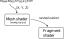
\includegraphics{figs/mesh_pipeline.svg.pdf}
    \end{center}

\end{frame}

%---------------------------------------------------------
\setLayout{vertical}
\begin{frame}{Mesh shading pipeline}

    \footnotesize

    \begin{center}
        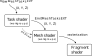
\includegraphics{figs/mesh_pipeline_with_task.svg.pdf}
    \end{center}

\end{frame}

%---------------------------------------------------------
\setLayout{vertical}
\begin{frame}{Mesh shading pipeline}

    \footnotesize

    \begin{center}
        \includegraphics{figs/mesh_pipeline_execution.svg.pdf}
    \end{center}

\end{frame}

%---------------------------------------------------------
\setLayout{vertical}
\begin{frame}{New shader stages}

    \LARGE

    \begin{block}{Task shader}
        How many mesh shader workgroups do you need? \\
        Optional "payload" output.
    \end{block}

    \begin{block}{Mesh shader}
        Uses a compute-like programming model to feed
        the rasterizer directly.
    \end{block}

\end{frame}

%---------------------------------------------------------
\setLayout{vertical}
\begin{frame}{Typical uses of mesh shading}

    \LARGE

    \begin{block}{Meshlets}
        During asset building, split your geometry into a smaller cluster of primitives: "meshlets". 
    \end{block}

    \begin{block}{Procedural geometry}
        Generate geometry on the fly according to a mathematical formula without loading any data from memory.
    \end{block}

\end{frame}

%---------------------------------------------------------
\setLayout{vertical}
\begin{frame}{What can you do in a task shader?}

    \LARGE

    \begin{itemize}
      	\item Coarse per-meshlet culling
      	\item LOD selection
      	\item Geometry amplification
      	\item Replacement for compute pre-pass
    \end{itemize}

\end{frame}

%---------------------------------------------------------
\setLayout{vertical}
\begin{frame}{What else can you do in a mesh shader?}

    \LARGE

    \begin{itemize}
      	\item Per-triangle culling
      	\item Procedural generation of vertices and primitives
    \end{itemize}

\end{frame}

\section{Mesa mesh shading implementation}

%---------------------------------------------------------
\setLayout{mainpoint}
{
\usebackgroundtemplate{
    \begin{picture}(100,256)(0,0)
        \put(0,0){
            \includegraphics[width=\paperwidth]{figs/road.jpg}
        }
        % Put the frame title in the middle of page
        \put(160,115){
            \begin{tabular}{m{0.7\textwidth}}
                \begin{flushleft}
                   \selectfont \Huge \bfseries \insertframetitle
                \end{flushleft}
            \end{tabular}
        }
        \put(150,80){
            \begin{tikzpicture}
                \fill[white] (0,0) rectangle (0.2,3);
            \end{tikzpicture}
        }
        \put(20,20){\pgfuseimage{logo2_medium}}
    \end{picture}
}
\begin{frame}{Mesa mesh shading implementation}
\end{frame}
}

%---------------------------------------------------------
\setLayout{vertical}
\begin{frame}{In the beginning... (September 2021)}

    \LARGE

    \begin{itemize}
      	\item NV\_mesh\_shader (no EXT)
      	\item No test cases (no CTS)
      	\item No users/apps (just an NV sample)
    \end{itemize}

\end{frame}

%---------------------------------------------------------
\setLayout{vertical}
\begin{frame}{RADV mesh shading progress}

    \LARGE

    \begin{itemize}
      	\item Oct-Dec 2021: \\ NV\_mesh\_shader mesh-only pipelines + VRS
      	\item Mar-Jun 2022: \\ Task shaders
      	\item Aug 2022: \\ EXT\_mesh\_shader
    \end{itemize}

\end{frame}

%---------------------------------------------------------
\setLayout{mainpoint}
\begin{frame}{}
    \frametitle{Mesh shaders \\ HW vs. programming model}
\end{frame}

%---------------------------------------------------------
\setLayout{vertical}
\begin{frame}{Where are outputs stored?}

    \LARGE

    \begin{itemize}
      	\item NVidia: shared memory
      	\item Intel: URB memory
      	\item AMD: export space
    \end{itemize}

\end{frame}

%---------------------------------------------------------
\setLayout{vertical}
\begin{frame}{AMD "NGG" HW limitations}

    \LARGE

    \begin{itemize}
      	\item 1 SIMD lane: up to 1 vertex + 1 primitive
      	\item Up to 32K shared memory per workgroup
      	\item 1D workgroup ID, etc.
    \end{itemize}

\end{frame}

%---------------------------------------------------------
\setLayout{vertical}
\begin{frame}{AMD "NGG" flow}

    \LARGE

    \begin{center}
        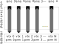
\includegraphics{figs/ms_ngg.svg.pdf}
    \end{center}

\end{frame}

%---------------------------------------------------------
\setLayout{vertical}
\begin{frame}{MS programming model requirements}

    \LARGE

    \begin{itemize}
      	\item Any invocation can write any vertex/primitive
      	\item Up to 48K shared memory per workgroup
      	\item 3D workgroup ID, etc.
    \end{itemize}

\end{frame}

%---------------------------------------------------------
\setLayout{vertical}
\begin{frame}{MS programming model requirements}

    \LARGE

    \begin{center}
        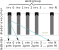
\includegraphics{figs/ms_model.svg.pdf}
    \end{center}

\end{frame}

%---------------------------------------------------------
\setLayout{vertical}
\begin{frame}{We can implement that using LDS (+ VRAM)}

    \LARGE

    \begin{center}
        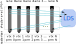
\includegraphics{figs/ms_ngg_lds.svg.pdf}
    \end{center}

\end{frame}

%---------------------------------------------------------
\setLayout{vertical}
\begin{frame}{Workgroup size vs. meshlet size}

    \LARGE

    \begin{center}
        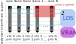
\includegraphics{figs/ms_ngg_full.svg.pdf}
    \end{center}

\end{frame}

%---------------------------------------------------------
\setLayout{mainpoint}
\begin{frame}{}
    \frametitle{Task shader implementation}
\end{frame}

%---------------------------------------------------------
\setLayout{vertical}
\begin{frame}{Task shader requirements}

    \LARGE

    \begin{itemize}
      	\item Dispatch mesh shader workgroups
      	\item Optional payload output up to 16K
      	\item Task/Mesh should run in parallel
    \end{itemize}

\end{frame}

%---------------------------------------------------------
\setLayout{vertical}
\begin{frame}{Task shader implementation ideas}

    \LARGE

    \begin{itemize}
      	\item Abuse the tessellator
      	\item Use a compute pre-pass
    \end{itemize}

\end{frame}

%---------------------------------------------------------
\setLayout{vertical}
\begin{frame}{Task shader implementation ideas}

    \LARGE

    \begin{itemize}
      	\item Abuse the tessellator (fixed func bottleneck)
      	\item Use a compute pre-pass (extra barrier)
    \end{itemize}

\end{frame}

%---------------------------------------------------------
\setLayout{vertical}
\begin{frame}{Task shader implementation ideas}

    \LARGE

    \begin{itemize}
      	\item Abuse the tessellator (Intel, NVidia)
      	\item Use a compute pre-pass
      	\item Do it in firmware (AMD)
    \end{itemize}

\end{frame}

%---------------------------------------------------------
\setLayout{vertical}
\begin{frame}{Task + mesh implementation on AMD}

    \LARGE
    Task shaders are graphics shaders, but the HW needs them
    to be executed on a different HW queue.

    \begin{itemize}
      	\item Mesh shaders: GFX queue (graphics / general)
      	\item Task shaders: ACE queue (async compute)
    \end{itemize}

\end{frame}

%---------------------------------------------------------
\setLayout{vertical}
\begin{frame}{Task + mesh implementation on AMD}

    \LARGE
    The difficulty is to pretend to the application that mesh/task are on the same queue.

\end{frame}

%---------------------------------------------------------
\setLayout{vertical}
\begin{frame}{Task + mesh implementation on AMD}

    \LARGE

    \begin{center}
        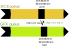
\includegraphics{figs/task_queues.svg.pdf}
    \end{center}

\end{frame}

%---------------------------------------------------------
\setLayout{vertical}
\begin{frame}{}

    \LARGE

    \begin{center}
        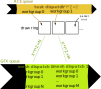
\includegraphics[height=8cm]{figs/task_queues_draw_ring.svg.pdf}
    \end{center}

\end{frame}

%---------------------------------------------------------
\setLayout{vertical}
\begin{frame}{}

    \LARGE

    \begin{center}
        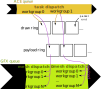
\includegraphics[height=8cm]{figs/task_queues_draw_payload_ring.svg.pdf}
    \end{center}

\end{frame}

%---------------------------------------------------------
\setLayout{mainpoint}
\begin{frame}{}
    \frametitle{Synchronizing the two queues}
\end{frame}

%---------------------------------------------------------
\setLayout{vertical}
\begin{frame}{ACE+GFX without synchronization}

    \LARGE

    \begin{center}
        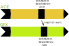
\includegraphics[height=6.75cm]{figs/task_sync_1.svg.pdf}
    \end{center}

\end{frame}

%---------------------------------------------------------
\setLayout{vertical}
\begin{frame}{What happens if you have a barrier?}

    \LARGE

    \begin{center}
        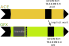
\includegraphics[height=6.75cm]{figs/task_sync_2.svg.pdf}
    \end{center}

\end{frame}

%---------------------------------------------------------
\setLayout{vertical}
\begin{frame}{What happens if you have a barrier?}

    \LARGE

    \begin{center}
        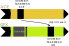
\includegraphics[height=6.75cm]{figs/task_sync_3.svg.pdf}
    \end{center}

\end{frame}

%---------------------------------------------------------
\setLayout{vertical}
\begin{frame}{What happens if you have a barrier?}

    \LARGE

    \begin{center}
        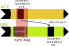
\includegraphics[height=6.75cm]{figs/task_sync_4.svg.pdf}
    \end{center}

\end{frame}

%---------------------------------------------------------
\setLayout{vertical}
\begin{frame}{Solving barriers with task shaders}

    \LARGE

    \begin{center}
        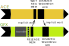
\includegraphics[height=6.75cm]{figs/task_sync_5.svg.pdf}
    \end{center}

\end{frame}

%---------------------------------------------------------
\setLayout{mainpoint}
\begin{frame}{}
    \frametitle{Multiple processes \\ with task shaders}
\end{frame}

%---------------------------------------------------------
\setLayout{vertical}
\begin{frame}{Optimal case with multiple processes}

    \LARGE

    \begin{center}
        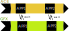
\includegraphics[height=5cm]{figs/task_deadlock_1.svg.pdf}
    \end{center}

\end{frame}

%---------------------------------------------------------
\setLayout{vertical}
\begin{frame}{But the kernel doesn't guarantee the ordering...}

    \LARGE

    \begin{center}
        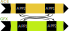
\includegraphics[height=5cm]{figs/task_deadlock_2.svg.pdf}
    \end{center}

\end{frame}

%---------------------------------------------------------
\setLayout{vertical}
\begin{frame}{But the kernel doesn't guarantee the ordering...}

    \LARGE

    \begin{center}
        
\includegraphics[height=5cm]{figs/task_deadlock_3.svg.pdf}
    \end{center}

\end{frame}

%---------------------------------------------------------
\setLayout{vertical}
\begin{frame}{But the kernel doesn't guarantee the ordering...}

    \LARGE

    Solution: "gang submit"
    
    \begin{itemize}
      \item Submit to multiple queues at the same time
      \item Kernel schedules the jobs together
      \item No mixup between different apps
    \end{itemize}

\end{frame}

%---------------------------------------------------------
\setLayout{vertical}
\begin{frame}{But the kernel doesn't guarantee the ordering...}

    \LARGE

    Solution: "gang submit"
    
    \begin{itemize}
      \item Not yet available in a released kernel
      \item Until then, \texttt{RADV\_PERFTEST=ext\_ms} \\
            (implemented with scheduled dependencies)
    \end{itemize}

\end{frame}

%---------------------------------------------------------
\setLayout{mainpoint}
\begin{frame}{}
    \frametitle{Where is the code?}
\end{frame}

%---------------------------------------------------------
\setLayout{vertical}
\begin{frame}{Where is the code?}

    \LARGE
    NIR lowering passes (backend specific)
    
    \begin{itemize}
      \item \texttt{ac\_nir\_lower\_ngg}
      \item \texttt{nir\_lower\_task\_shader}
      \item \texttt{ac\_nir\_lower\_taskmesh\_io\_to\_mem}
    \end{itemize}

\end{frame}

%---------------------------------------------------------
\setLayout{vertical}
\begin{frame}{Where is the code?}

    \LARGE
    RADV code
    
    \begin{itemize}
      \item \texttt{radv\_pipeline}
      \item \texttt{radv\_cmd\_buffer}
      \item Major refactor in the submission code
    \end{itemize}

\end{frame}

\section{Demo}

%---------------------------------------------------------
\setLayout{mainpoint}
\begin{frame}{}
    \frametitle{Demo}
\end{frame}

%---------------------------------------------------------
\setLayout{vertical}
\begin{frame}{Mesh shading demo}

    \LARGE

    NVidia CAD scene demo \\
    The scene contains nine cars, but the camera focuses on a single one,
    most others are fully outside frustum. The total scene has 32 M triangles and 16 K drawcalls.

\end{frame}

%---------------------------------------------------------
\setLayout{blank}
{
    \usebackgroundtemplate{\includegraphics[width=\paperwidth]{figs/squirrel.jpg}}%
    \begin{frame}

        \vspace{2cm}
        
        \textbf{\Huge Thanks}
        
        \ \\
        
        \textbf{\LARGE Questions, suggestions, discussion?}
        
        \ \\
        
        \textbf{\normalsize Mesh shading implementation in Mesa}
        \ \\
        
        \text{\normalsize Timur Kristóf}
        
        \ \\
        
        \text{\footnotesize Venemo @ \#dri-devel, \#radeon, ...}
        \ \\
        \text{\footnotesize https://timur.hu}
        \ \\
        \ \\
        \ \\
        \ \\
        \text{\footnotesize https://github.com/Venemo/xdc2022\_mesa\_mesh\_shading}
        
        \vspace{1.4cm}
        \includegraphics[height=1cm]{lib/logos/valve_logo.pdf}
        
    \end{frame}
}

%---------------------------------------------------------
\setLayout{titlepage}
\titlepage

\end{document}
